%%%%%%%%%%%%%%%%%%%%%%%%%%%%%%%%%%%%%%%%%%%%%%%%%%%%%%%%%%%%%%%%%%%%%
% LaTeX Template: Project Titlepage Modified (v 0.1) by rcx
%
% Original Source: http://www.howtotex.com
% Date: February 2014
% 
% This is a title page template which be used for articles & reports.
% 
% This is the modified version of the original Latex template from
% aforementioned website.
% 
%%%%%%%%%%%%%%%%%%%%%%%%%%%%%%%%%%%%%%%%%%%%%%%%%%%%%%%%%%%%%%%%%%%%%%

\documentclass[12pt]{report}
\usepackage[a4paper]{geometry}
\usepackage[utf8]{inputenc}
\usepackage[myheadings]{fullpage}
\usepackage{fancyhdr}
\usepackage{lastpage}
\usepackage{graphicx, wrapfig, subcaption, setspace, booktabs}
\usepackage[T1]{fontenc}
\usepackage[font=small, labelfont=bf]{caption}
\usepackage{fourier}
\usepackage[protrusion=true, expansion=true]{microtype}
\usepackage[english]{babel}
\usepackage{sectsty}
\usepackage{url, lipsum}
\usepackage{listings}
\usepackage{hyperref}

\usepackage{color}

\definecolor{codegreen}{rgb}{0,0.6,0}
\definecolor{codegray}{rgb}{0.5,0.5,0.5}
\definecolor{codepurple}{rgb}{0.58,0,0.82}
\definecolor{backcolour}{rgb}{0.95,0.95,0.92}

\lstdefinestyle{codigo}{
    backgroundcolor=\color{backcolour},   
    commentstyle=\color{codegreen},
    keywordstyle=\color{magenta},
    numberstyle=\tiny\color{codegray},
    stringstyle=\color{codepurple},
    basicstyle=\footnotesize,
    breakatwhitespace=false,         
    breaklines=true,                 
    captionpos=b,                    
    keepspaces=true,                 
    numbers=left,                    
    numbersep=3pt,                  
    showspaces=false,                
    showstringspaces=false,
    showtabs=false,                  
    tabsize=2
}

\lstset{style=codigo}

\newcommand{\HRule}[1]{\rule{\linewidth}{#1}}
\onehalfspacing
\setcounter{tocdepth}{5}
\setcounter{secnumdepth}{5}

%-------------------------------------------------------------------------------
% HEADER & FOOTER
%-------------------------------------------------------------------------------
\pagestyle{fancy}
\fancyhf{}
\setlength\headheight{15pt}
\fancyhead[L]{Toledo Margalef, Pablo Adrian}
\fancyhead[R]{Base de Datos II - UNPSJB}
\fancyfoot[R]{\thepage}
%-------------------------------------------------------------------------------
% TITLE PAGE
%-------------------------------------------------------------------------------

\begin{document}

\title{ \normalsize \textsc{Laboratorio I}
    \\ [2.0cm]
    \HRule{0.5pt} \\
    \LARGE \textbf{\uppercase{PL/PGSQL, PROCESAMIENTO Y OPTIMIZACIÓN DE CONSULTAS}}
\HRule{2pt} \\ [0.5cm]}


\author{
    Cátedra: \\
    Lic. Ingravallo, Gabriel\\
    Lic. Parise, Cristian\\
    Integrantes: \\
    Toledo Margalef, Pablo Adrían \\ 
Universidad Nacional de la Patagonia San Juan Bosco}

\maketitle
\newpage

%-------------------------------------------------------------------------------
% Section title formatting
\sectionfont{\scshape}
%-------------------------------------------------------------------------------

%-------------------------------------------------------------------------------
% BODY
%-------------------------------------------------------------------------------

\section*{Consigna Planteada}

\begin{enumerate}
    \item Agregar tuplas en forma masiva a las tablas modeloAvion y Avion de forma tal que por cada modeloAvion insertado se agreguen 10000 aviones y que la estadística \\$V(capacidad, modeloAvion) \geq 1000$. Además por cada avión agregado agregar una reparación del mismo (con algún DNI de trabajador ya preexistente). Se debe
        presentar el script de la solucion.
    \item Hacer una selección de las reparaciones para aviones cuya capacidad es = X (tomar para X un valor válido de los que se encuentren en su base de datos) Analizar el plan de ejecución de la consulta del punto anterior. Documentar en su informe
    \item Podría cambiar en algo el esquema físico de la base de datos de forma tal que se consiga algún plan de ejecución que acelere la consulta
    \item Implementar el cambio propuesto en el punto 4
    \item Volver a analizar la consulta del punto 2, viendo si el plan de ejecución cambió. Documentar el nuevo plan logrado y comparar con el anterior explicando los cambios encontrados.
\end{enumerate}

\newpage

\section*{Generación del script}

Para poder cumplir con la consigna planteada se plantearon las siguientes necesidades.

\begin{enumerate}
    \item Generar un conjunto inicial de Trabajadores
    \item Generar un conjunto inicial de Modelos de Avión
    \item Generar un conjunto inicial de Fallas
\end{enumerate}

Para poder contar con datos a partir de los cuales poder accionar el script y popular la base con registros de Avión y de Reparaciones.

\subsection*{Datos de base para el script}

En el caso de los empleados, se utilizó el sitio web  \href{https://www.json-generator.com/}{JSON Generator}  para poder generar un conjunto de trabajadores con los campos que correspondieran con los de la tabla Trabajador. Luego se utilizó un script en Python para poder generar, a partir del JSON, un script sql para alimentar al motor.

El script resultante contiene columnas del estilo;


\begin{lstlisting}[language=SQL]
insert into trabajador values (15000000,'Lee Kemp','Coventry Road 7874',148,'(935)425-2782',261);
\end{lstlisting}


Luego, para solventar la necesidad de modelos de avión a partir de los cuales generar aviones dentro del scritp. Se recurrió al siguiente dataset de \href{https://www.kaggle.com/saurograndi/airplane-crashes-since-1908/data}{Accidentes Aéreos} para poder extraer los nombres de los modelos. Luego se creó una tabla adicional "descripcionModelo", conteniendo como único campo el nombre del modelo, esta relación se va a utilizar en la función requerida para poblar la base de aviones y reparaciones.

Para poder generar el conjunto de fallas a incluir en cada reparación se utilizó el siguiente dataset de \href{https://www.kaggle.com/rtatman/lego-database/data}{Partes de Piezas Lego} para extraer nombres de partes y contar con nombres que se pudieran usar en la descripción de cada falla.

Se obtuvo un script con la siguiete forma:

\begin{lstlisting}[language=SQL]
insert into falla values (10,'Set 0687 Activity Booklet 1');
\end{lstlisting}

Ya con todos estos elementos, se dispuso a generar la función de carga.

Se detalla a continuación:

\begin{lstlisting}[language=SQL]
create or replace function laboratorio1() returns void as
$$
declare
model record;
modelo record;
i integer;
capacidad integer;
tipoModelo integer;
nro_avion integer;
horas_vuelo integer;
anio integer;
fecha_inicio date;
fecha_fin date;
trabajador integer;
falla integer;
begin
    tipoModelo=20;
    capacidad = 100;

    -- creamos modelos de avion
    for model in (select * from "descripcionModeloAviones") loop
        -- Insertar modelo con la descripcion 
        -- que hay en otra tabla
        insert into "modeloAvion" values (tipoModelo, model.model, capacidad);
        tipoModelo = tipoModelo +1;
        capacidad = capacidad +1;
    end loop;

    fecha_inicio = current_date;
    fecha_fin = fecha_inicio + 20;
    nro_avion = 1050;

    -- por cada modelo
    for modelo in (select * from "modeloAvion") loop
        raise notice 'En el modelo %',modelo."tipoModelo";
        -- se crean los 10000 aviones con una reparacion cada uno
        for i in 1..10000 loop

            -- Horas de vuelo
            horas_vuelo = floor(random()*(5000-300+1))+300;

            -- Anio de fabricacion del avion
            anio = floor(random()*(2010-1990+1))+1990;

            -- DNI del trabajador de la reparacion
            trabajador = floor(random()*(15000999-15000001+1))+15000001;

            -- Codigo de la falla
            falla = floor(random()*(287-10+1))+10;

            -- Insertamos avion
            insert into avion values (nro_avion, modelo."tipoModelo",anio, horas_vuelo);

            -- Insertamos reparacion
            insert into "trabajadorReparacion" values (trabajador, nro_avion, fecha_inicio, fecha_fin, falla);

            -- Incrementamos nro de avion
            nro_avion = nro_avion + 1;

            end loop;
            end loop;
            end;
            $$ language plpgsql;

            select laboratorio1();
\end{lstlisting}

Luego de que la función finalizó su ejecución se ejecutó la siguiente consulta (escrita a partir del enunciado planteado en un principio):

\begin{lstlisting}[language=SQL]
select
tav."nroAvion",
tav."dniTrabajador",
tav."fechaInicioReparacion",
tav."fechaFinReparacion",
falla."descripcion"
from 
"trabajadorReparacion" tav
join 
avion on avion."nroAvion"=tav."nroAvion"
join
"modeloAvion" ma on avion."tipoModelo" = ma."tipoModelo"
join
falla on falla."tipoFalla" = tav."tipoFallaReparada"
where
ma.capacidad = 1388;
\end{lstlisting}

Se extrajo luego el siguiente plan de ejecución

\begin{lstlisting}
Hash Join  (cost=466017.33..955422.38 rows=10000 width=67) (actual time=5195.045..6928.601 rows=10000 loops=1)
  Output: tav."nroAvion", tav."dniTrabajador", tav."fechaInicioReparacion", tav."fechaFinReparacion", falla.descripcion
  Hash Cond: (tav."tipoFallaReparada" = falla."tipoFalla")
  Buffers: shared hit=886 read=285515
  ->  Hash Join  (cost=466007.98..955275.54 rows=10000 width=20) (actual time=5194.674..6926.688 rows=10000 loops=1)
        Output: tav."nroAvion", tav."dniTrabajador", tav."fechaInicioReparacion", tav."fechaFinReparacion", tav."tipoFallaReparada"
        Hash Cond: (tav."nroAvion" = avion."nroAvion")
        Buffers: shared hit=880 read=285515
        ->  Seq Scan on public."trabajadorReparacion" tav  (cost=0.00..398005.04 rows=24310004 width=20) (actual time=0.045..1701.718 rows=24310004 loops=1)
              Output: tav."dniTrabajador", tav."nroAvion", tav."fechaInicioReparacion", tav."fechaFinReparacion", tav."tipoFallaReparada"
              Buffers: shared hit=290 read=154615
        ->  Hash  (cost=465882.98..465882.98 rows=10000 width=4) (actual time=3206.657..3206.657 rows=10000 loops=1)
              Output: avion."nroAvion"
              Buckets: 16384  Batches: 1  Memory Usage: 480kB
              Buffers: shared hit=590 read=130900
              ->  Hash Join  (cost=114.40..465882.98 rows=10000 width=4) (actual time=1736.240..3205.609 rows=10000 loops=1)
                    Output: avion."nroAvion"
                    Hash Cond: (avion."tipoModelo" = ma."tipoModelo")
                    Buffers: shared hit=590 read=130900
                    ->  Seq Scan on public.avion  (cost=0.00..374506.06 rows=24310006 width=8) (actual time=0.015..1592.865 rows=24310006 loops=1)
                          Output: avion."nroAvion", avion."tipoModelo",avion."anio", avion."horasVuelo"
                          Buffers: shared hit=506 read=130900
                    ->  Hash  (cost=114.39..114.39 rows=1 width=4) (actual time=1.085..1.085 rows=1 loops=1)
                          Output: ma."tipoModelo"
                          Buckets: 1024  Batches: 1  Memory Usage: 9kB
                          Buffers: shared hit=84
                          ->  Seq Scan on public."modeloAvion" ma  (cost=0.00..114.39 rows=1 width=4) (actual time=0.645..1.074 rows=1 loops=1)
                                Output: ma."tipoModelo"
                                Filter: (ma.capacidad = 1388)
                                Rows Removed by Filter: 2430
                                Buffers: shared hit=84
  ->  Hash  (cost=5.82..5.82 rows=282 width=55) (actual time=0.320..0.320 rows=282 loops=1)
        Output: falla.descripcion, falla."tipoFalla"
        Buckets: 1024  Batches: 1  Memory Usage: 33kB
        Buffers: shared hit=3
        ->  Seq Scan on public.falla  (cost=0.00..5.82 rows=282 width=55) (actual time=0.028..0.138 rows=282 loops=1)
              Output: falla.descripcion, falla."tipoFalla"
              Buffers: shared hit=3
Planning time: 2.689 ms
Execution time: 6929.100 ms
\end{lstlisting}

Con la ayuda de la herramienta \href{http://tatiyants.com/pev/}{Postgres EXPLAIN Visualizer} se grafica el plan de aplicación obtenido (Figure 1).

\begin{figure}[!ht]
    \centering
    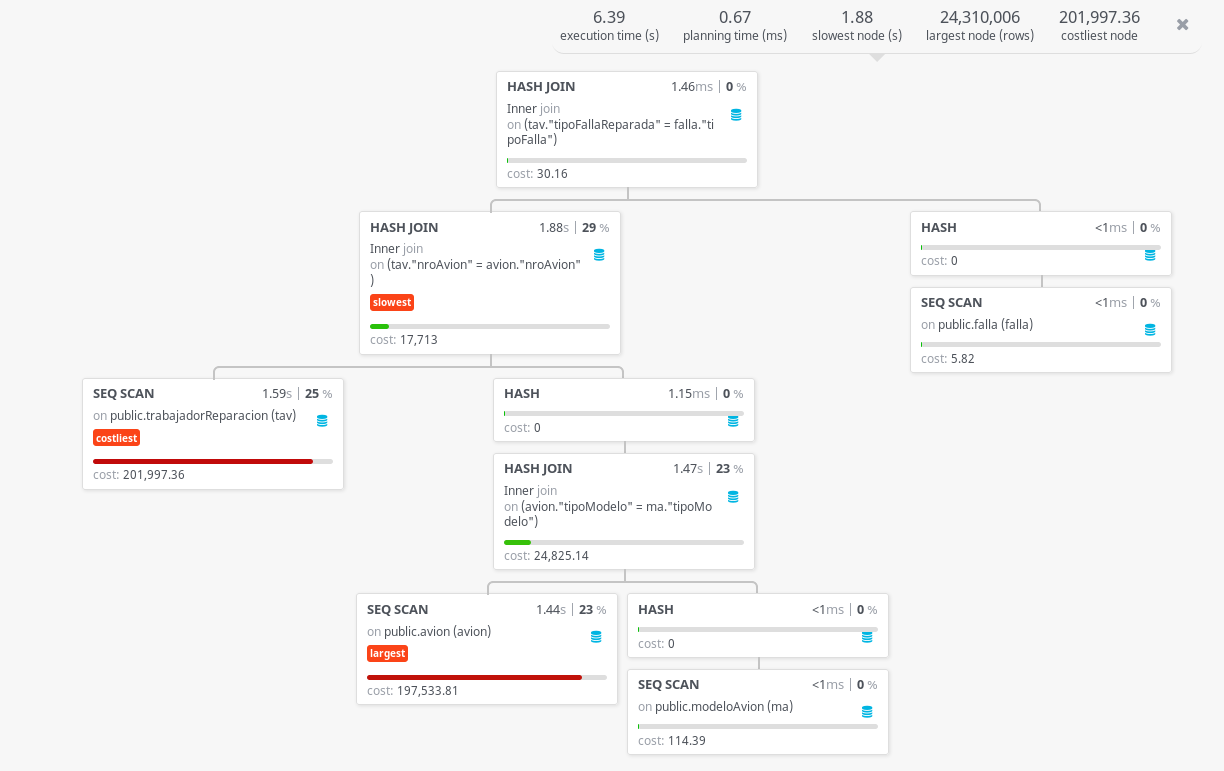
\includegraphics[width=1\textwidth]{images/plan_ejecucion_pre_index.png}
    \caption{Plan de Ejecucion}
    \centering
    \label{label:file_name}
\end{figure}

Observamos que los costos de ambos \textbf{SEQ SCAN} son extremadamente elevados. Por lo tanto se propone la creación de dos índices, uno sobre la columna "nroAvion" de Avion (Indice sobre campo clave) y otro sobre la columns "nroAvion" (indice secundario) de trabajadorReparacion.

\begin{lstlisting}[language=SQL]
create unique index "avionesNroAvion" on avion("nroAvion");
create index "reparacionesAvion" on "trabajadorReparacion"("nroAvion")
\end{lstlisting}

Repetimos la consulta, obtenemos el plan de aplicación y lo graficamos nuevamente (Figure 2)

\begin{figure}[!ht]
    \centering
    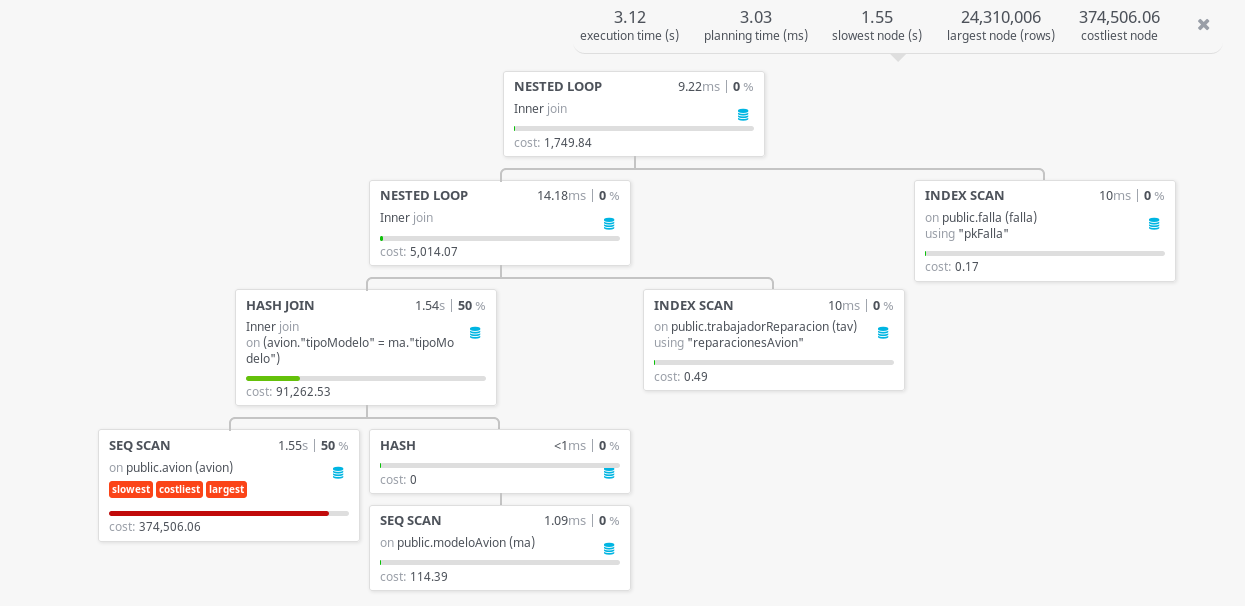
\includegraphics[width=1\textwidth]{images/plan_ejecucion_index_1.png}
    \caption{Plan de Ejecucion luego de crear el primer índice}
    \centering
    \label{label:file_name}
\end{figure}

Observamos que los costos se redujeron drásticamente en todos los nodos, pero todavía nos queda ese nodo de búsqueda secuencial que tiene un costo elevadísimo que luego participa del join con la tabla modeloAvion. Se procede a crear un índice (secundario) sobre la columna "tipoModelo" de la tabla Avion.

\begin{lstlisting}[language=SQL]
create index "avionesModelo" on avion("tipoModelo");
\end{lstlisting}

Repetimos la consulta, obtenemos el plan de aplicación y lo graficamos nuevamente (Figure 3)

\begin{figure}[!ht]
    \centering
    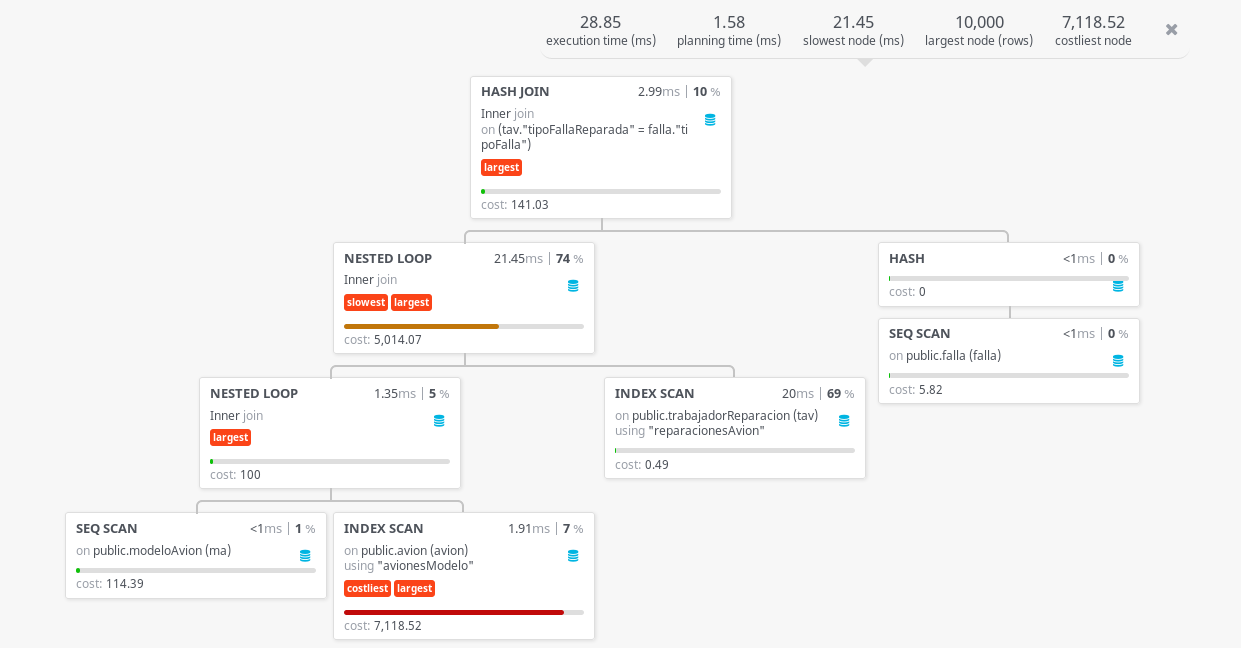
\includegraphics[width=1\textwidth]{images/plan_ejecucion_index_2.png}
    \caption{Plan de Ejecucion luego de crear el segundo índice}
    \centering
    \label{label:file_name}
\end{figure}

El costo de a búsqueda en la tabla de aviones sigue siendo de los más elevados, pero no podemos dejar de lado que con respecto al plan de ejecución anterior bajo de un costo de 374506,6 a tan solo 7118,52, es decir que disminuyó aproximadamente un 98\%

De esta forma se pudo ver cómo al modificar un elemento del esquema físico, como ser un índice sobre un campo de una tabla y sin modificar en nada la consulta realizada se observaron mejorar muy importantes en los tiempos de respuesta del motor.


En la siguiente tabla (Table 1) se ilustran las diferencias en tiempo en los diferentes cambios que se le aplicaron al motor, luego una gráfica de tiempo con respecto a la cantidad de índices (Figure 4).


\begin{table}[!ht]\footnotesize
   \centering
   \begin{tabular}{cccccc}
   \toprule
   \multicolumn{6}{c} {Tiempo de consulta} \\
   \midrule    
   \multicolumn{2}{c} {Sin índices} & \multicolumn{2}{c} {Primeros dos índices} & \multicolumn{2}{c} {Tercer índice} \\
   \midrule
   Males & Females & 1st level & 6th level & Males & Females \\
   \midrule
   \multicolumn{2}{c} {6.39s} & \multicolumn{2}{c} {3.12s} & \multicolumn{2}{c} {28.85ms} \\
   \bottomrule
   \end{tabular}
   \caption{}
   \label{label:tests}
\end{table}

\begin{figure}[!ht]
    \centering
    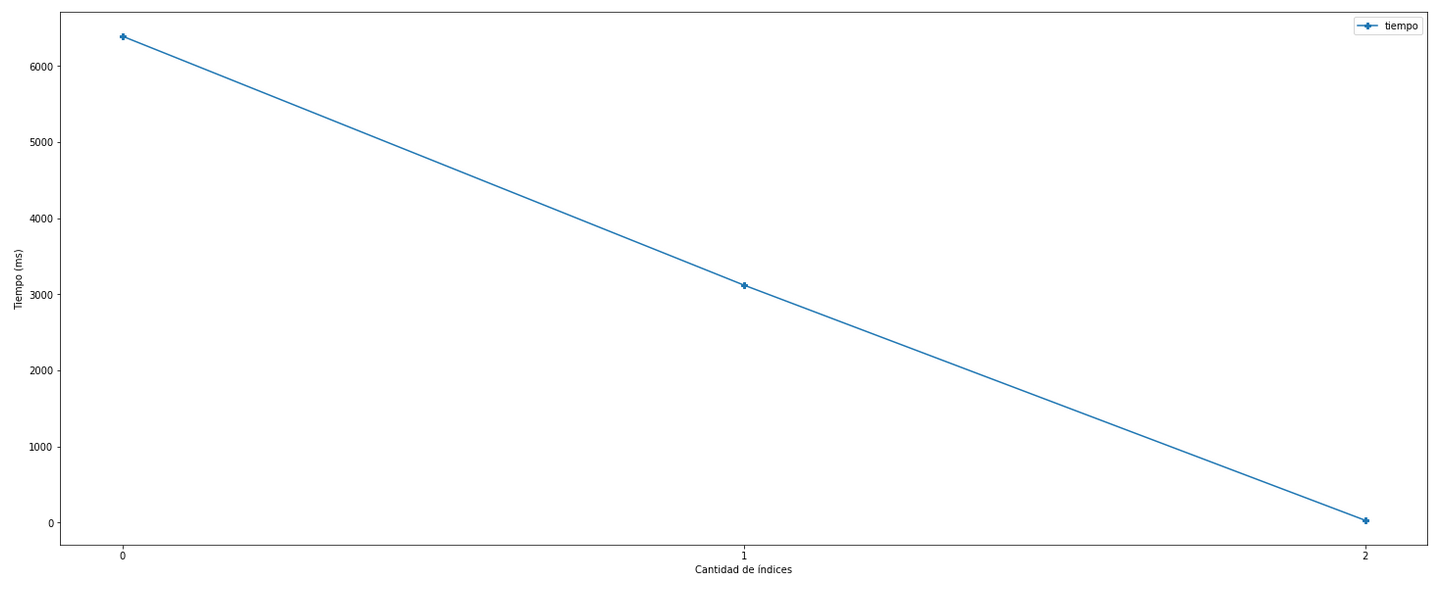
\includegraphics[width=1\textwidth]{images/tiempo.png}
    \caption{Comparación de tiempos ante la presencia de los diferentes índices creados}
    \centering
    \label{label:file_name}
\end{figure}
%-------------------------------------------------------------------------------
% REFERENCES
%-------------------------------------------------------------------------------

\end{document}

%-------------------------------------------------------------------------------
% SNIPPETS
%-------------------------------------------------------------------------------

%\begin{figure}[!ht]
%   \centering
%   \includegraphics[width=0.8\textwidth]{file_name}
%   \caption{}
%   \centering
%   \label{label:file_name}
%\end{figure}

%\begin{figure}[!ht]
%   \centering
%   \includegraphics[width=0.8\textwidth]{graph}
%   \caption{Blood pressure ranges and associated level of hypertension (American Heart Association, 2013).}
%   \centering
%   \label{label:graph}
%\end{figure}

%\begin{wrapfigure}{r}{0.30\textwidth}
%   \vspace{-40pt}
%   \begin{center}
%       \includegraphics[width=0.29\textwidth]{file_name}
%   \end{center}
%   \vspace{-20pt}
%   \caption{}
%   \label{label:file_name}
%\end{wrapfigure}

%\begin{wrapfigure}{r}{0.45\textwidth}
%   \begin{center}
%       \includegraphics[width=0.29\textwidth]{manometer}
%   \end{center}
%   \caption{Aneroid sphygmomanometer with stethoscope (Medicalexpo, 2012).}
%   \label{label:manometer}
%\end{wrapfigure}

%\begin{table}[!ht]\footnotesize
%   \centering
%   \begin{tabular}{cccccc}
%   \toprule
%   \multicolumn{2}{c} {Pearson's correlation test} & \multicolumn{4}{c} {Independent t-test} \\
%   \midrule    
%   \multicolumn{2}{c} {Gender} & \multicolumn{2}{c} {Activity level} & \multicolumn{2}{c} {Gender} \\
%   \midrule
%   Males & Females & 1st level & 6th level & Males & Females \\
%   \midrule
%   \multicolumn{2}{c} {BMI vs. SP} & \multicolumn{2}{c} {Systolic pressure} & \multicolumn{2}{c} {Systolic Pressure} \\
%   \multicolumn{2}{c} {BMI vs. DP} & \multicolumn{2}{c} {Diastolic pressure} & \multicolumn{2}{c} {Diastolic pressure} \\
%   \multicolumn{2}{c} {BMI vs. MAP} & \multicolumn{2}{c} {MAP} & \multicolumn{2}{c} {MAP} \\
%   \multicolumn{2}{c} {W:H ratio vs. SP} & \multicolumn{2}{c} {BMI} & \multicolumn{2}{c} {BMI} \\
%   \multicolumn{2}{c} {W:H ratio vs. DP} & \multicolumn{2}{c} {W:H ratio} & \multicolumn{2}{c} {W:H ratio} \\
%   \multicolumn{2}{c} {W:H ratio vs. MAP} & \multicolumn{2}{c} {\% Body fat} & \multicolumn{2}{c} {\% Body fat} \\
%   \multicolumn{2}{c} {} & \multicolumn{2}{c} {Height} & \multicolumn{2}{c} {Height} \\
%   \multicolumn{2}{c} {} & \multicolumn{2}{c} {Weight} & \multicolumn{2}{c} {Weight} \\
%   \multicolumn{2}{c} {} & \multicolumn{2}{c} {Heart rate} & \multicolumn{2}{c} {Heart rate} \\
%   \bottomrule
%   \end{tabular}
%   \caption{Parameters that were analysed and related statistical test performed for current study. BMI - body mass index; SP - systolic pressure; DP - diastolic pressure; MAP - mean arterial pressure; W:H ratio - waist to hip ratio.}
%   \label{label:tests}
%\end{table}


